% !TEX root = thesis-ex.tex

%The quark gluon plasma is a strongly coupled medium \cite{} that is produced in a heavy ion collision. This section will briefly describe the heavy ion environment it is formed in and subsequently the medium itself. 

In a heavy ion collision, each incident nucleus is a lorentz contracted disc. In the case of a \pbpb\ collision, the nuclei have been accelerated to energies where the relativistic $\gamma$ factor is between 100 and 2500 for beam rapidities of $y = 5.3$ and 8.5. 
%The partons within each nucleons are sources of transverse color fields

When these pancake like discs collide, most of the partons are participate in soft interactions that do not involve large transverse momentum transfer, and are hence scattered only at small angles. A small fraction of the colliding partons however do undergo hard perturbative interactions and lead to particles with large transverse momenta.

While the maximum energy density in the process occurs just at the collision, the energy density 1 fm/c after the collision is 12 $\mathrm{GeV} / \mathrm{fm}^3$, much higher than the 500 $\mathrm{MeV} / \mathrm{fm}^3$ in a typical hadron. Lattice QCD calculations in thermodynamics show that at these energies, the partons produced in the collision cannot be treated as a collection of distinct hadrons. In fact, these partons are strongly coupled to each other \cite{???} , forming a medium that can be described by relativistic hydrodynamics. This medium, called the quark gluon plasma (QGP) has a viscosity to entropy ratio that is almost at the theoretical minimum of of $\eta / S = 1/4\pi$ \cite{5,6, check126}. 

After the collision and as the nuclei are receding from each other, the energy density between them starts to decrease as the QGP cools and expands. This process can be seen in Figure~\ref{fig:qgp_form}. Once formed, the QGP hydrodynamically flows, with the initial pressure driving the expansion and the subsequent cooling. This continues till the energy density drops to below that within a hadron and the fluid hadronizes. These individual hadrons briefly scatter off of each other before they freely fly towards the detector (freezeout).
% It is to be noted that there is QGP continuously formed in the wake of the nuclei since the partons produced at large rapidities are highly relativistic and 

\begin{figure}[htbp]
\begin{center}
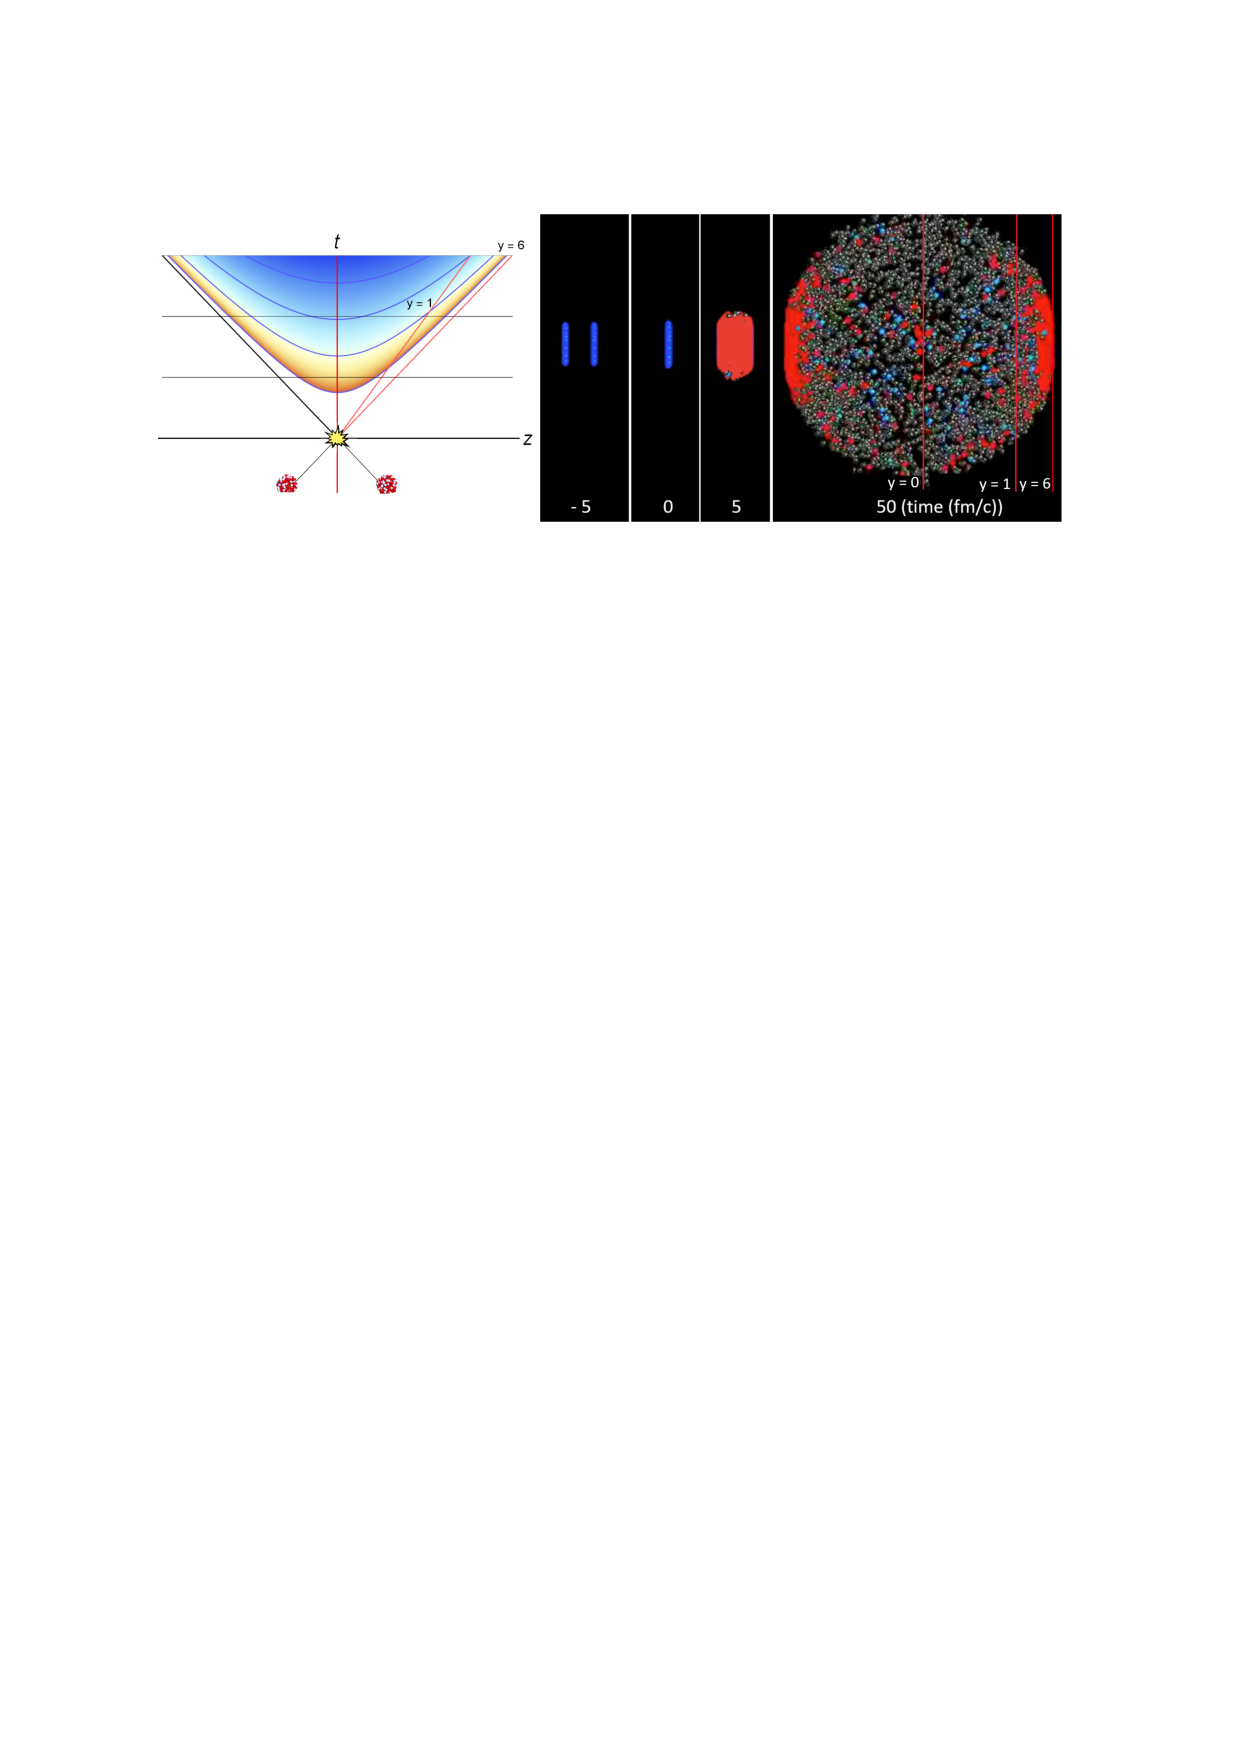
\includegraphics[width=0.85\textwidth]{figures/theory/qgp_formation}
\caption{(left) Space-time diagram for a heavy ion collision. The color is indicative of the temperature of the QGP formed. (right) Snapshots of a heavy ion collision at $\sqrtsnn = 2.76$ TeV at different times. The Lorentz contracted nuclei are in blue while the QGP is in red. Figures from References \cite{7, 8}.  }
\label{fig:qgp_form}
\end{center}
\end{figure}

While Figure~\ref{fig:qgp_form} shows snapshots of a head on (central) collision between two large nuclei, it is possible to have collisions where the impact parameter is larger and hence the overlap region is smaller. These collisions, called peripheral collisions, qualitatively undergo the same process described above, with the size and shape of the QGP being different. In these collisions, the QGP formed is more lenticular in the transverse direction. Variations in the shape of the QGP due to the collision centrality result in pressure gradients that further cause azimuthal anisotropies in the momentum distribution of the produced particles. 

%We can differentiate different nucleons in the collision as per the following:
%\subparagraph{$\mathrm{N}_{\mathrm{part}}$: } This is the number nucleons that have collided with at least one other nucleon, and can be said to have participated in the heavy ion collision.
%\subparagraph{$\mathrm{N}_{\mathrm{coll}}$: } This is the number of binary collisions that take place between the nucleons of the colliding nuclei. It is typically much larger than \Npart.
%\subparagraph{$\mathrm{N}_{\mathrm{spec}}$: } This is the number nucleons that do not encounter any nucleon from the other nucleus and are just spectators to the collision. 


%The properties of the QGP can be determined by azimuthal correlation measurements \cite{5, 6, 90}, while how it interacts with a high energy parton can be determined by jet studies \cite{91, 92, 69, etc}. 

\subsection{The Quark Gluon Plasma}
At the peak energy density of the collision, the system cannot be described at the level of hadrons, and has to be described in terms of quarks and gluons. The initial anisotropic energy density being reflected in the azimuthal variation of particle production implies a strongly coupled medium that expands hydrodynamically, with a faster expansion in the direction of larger gradients and hence resulting a momentum anisotropy. See \cite{116, 117, 118, 63}.

Azimuthal correlation measurements \cite{5?, 6?, 90?, 110?, 111?} indicated the momentum anisotropy in the collision is  remains, implying that the medium is strongly coupled. 

A Fourier Transform of the angular distribution of charged hadrons in the collision debris can quantify these measurements and give the anisotropic flow coefficients $v_n$, defined as \cite{115}:

\begin{align}
\frac{d\bar{N}}{d\phi} = \frac{\bar{N}}{2\pi} \left( 1 + 2 \sum_{n=1}^{\inf} v_{n} \cos(n(\phi-\bar{\Psi}_n)) \right)
\end{align}

where $\phi$ is the angle in the transverse plane, $\bar{\Psi}_n$ are the event plane angles, and $\bar{N}$ is the average number of particles per event. Some of these coefficients are shown in Figure~\ref{fig:flow_coeff}.


\begin{figure}[htbp]
\begin{center}
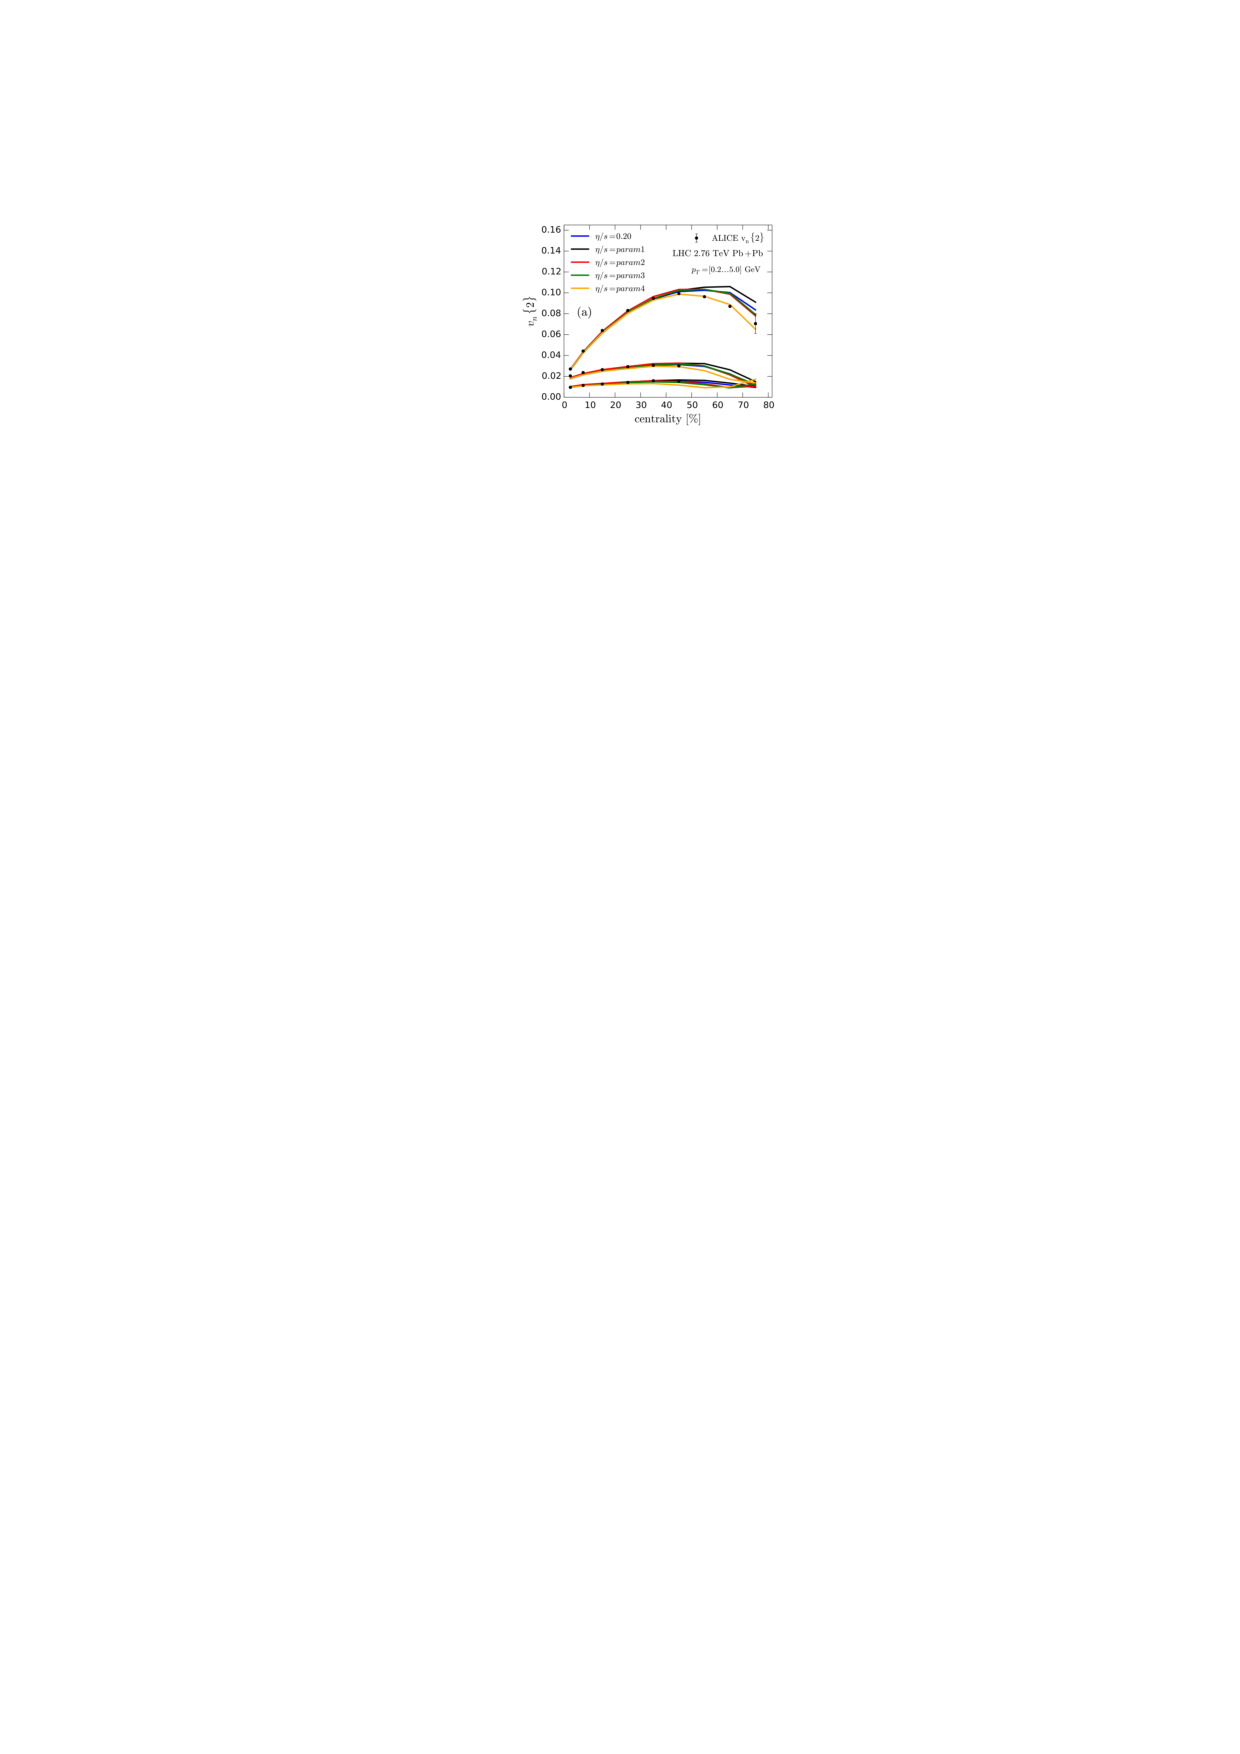
\includegraphics[width=0.65\textwidth]{figures/theory/flow_coefficients}
\caption{Comparison of a hydrodynamic model from \cite{107} to the anisotropy measurements by ALICE \cite{108} for different parameterizations of the $\eta/s$ and for different $v_n (n = 2, 3, 4)$ from top to bottom as a function of collision centrality.  -- see ATLAS measurement from \cite{109}.}
\label{fig:flow_coeff}
\end{center}
\end{figure}



